\documentclass[conference]{IEEEtran}
\IEEEoverridecommandlockouts
\usepackage{cite}
\usepackage{amsmath,amssymb,amsfonts}
\usepackage{algorithmic}
\usepackage{graphicx}
\usepackage{textcomp}
\usepackage{xcolor}
\usepackage{subcaption}
\def\BibTeX{{\rm B\kern-.05em{\sc i\kern-.025em b}\kern-.08em
    T\kern-.1667em\lower.7ex\hbox{E}\kern-.125emX}}

\begin{document}

\title{Low-Latency Federated Learning over Wireless Networks\\
\thanks{This work was supported by Grant 12345.}}

\author{\IEEEauthorblockN{1\textsuperscript{st} Ana Silva}
\IEEEauthorblockA{\textit{Dept. of Electrical Engineering} \\
\textit{Example University}\\
Lisbon, Portugal \\
ana@example.pt}
\and
\IEEEauthorblockN{2\textsuperscript{nd} Ben Okoro}
\IEEEauthorblockA{\textit{School of Computing} \\
\textit{Tech Institute}\\
Lagos, Nigeria \\
ben@example.ng}
}

\maketitle

\begin{abstract}
We propose a scheduling scheme that reduces round latency by 35\%.
\end{abstract}

\begin{IEEEkeywords}
federated learning, scheduling, wireless
\end{IEEEkeywords}

\section{Introduction}
\IEEEPARstart{F}{ederated} learning (FL) trains models across devices~\cite{smith2020,lee2019}.
Prior work~\cite{knuth1984} ignored channel state.

\section{System Model}
Each device $k$ has bandwidth $B_k$ and the rate is
\begin{equation}
R_k = B_k \log_2\left(1 + \frac{p_k |h_k|^2}{N_0 B_k}\right). \label{eq:rate}
\end{equation}

\begin{figure}[htbp]
\centering
\begin{subfigure}[b]{0.48\columnwidth}
  \centering
  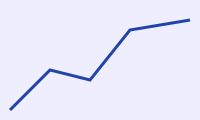
\includegraphics[width=\linewidth]{plot.svg}
  \caption{Latency}
  \label{fig:lat}
\end{subfigure}
\hfill
\begin{subfigure}[b]{0.48\columnwidth}
  \centering
  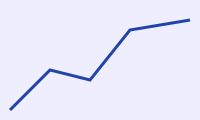
\includegraphics[width=\linewidth]{diagram.svg}
  \caption{Accuracy}
  \label{fig:acc}
\end{subfigure}
\caption{Results: (a) latency and (b) accuracy.}
\label{fig:results}
\end{figure}

Fig.~\ref{fig:results} and Fig.~\subref{fig:lat} show the gains.

\begin{algorithmic}[1]
\REQUIRE devices $\mathcal{K}$
\FOR{each round $t$}
\STATE select subset $S_t$
\IF{$|S_t| = 0$}
\STATE \textbf{break}
\ENDIF
\ENDFOR
\RETURN model
\end{algorithmic}

\section{Conclusion}
The scheme is practical.

\bibliographystyle{IEEEtran}
\bibliography{refs}
\end{document}
